\section{Results}

To analyse the measured data, the Python \cite{python} packages NumPy \cite{numpy} and SciPy \cite{scipy} are used, with Matplotlib
\cite{matplotlib} generating the graphical presentation and Uncertainties \cite{uncertainties} allowing for automated linear order
propagation of errors obtained from fit functions. The code is included in the appendix.



\subsection{Adjustment}

A modified Gaussian distribution of the form
\begin{equation*}
	G(\alpha_i; a, b, \mu, \sigma) = a e^{-(\alpha_i - \mu)^2 / 2\sigma^2} + b
\end{equation*}
is fitted to the primary beam profile, where $a$ and $b$ account for the amplitude and background, respectively. Since the intensity
$I$ is given in arbitrary units, it is normalized via $I \rightarrow I / I_\text{max}$ for all following measurements.

\begin{figure}[H]
	\centering
	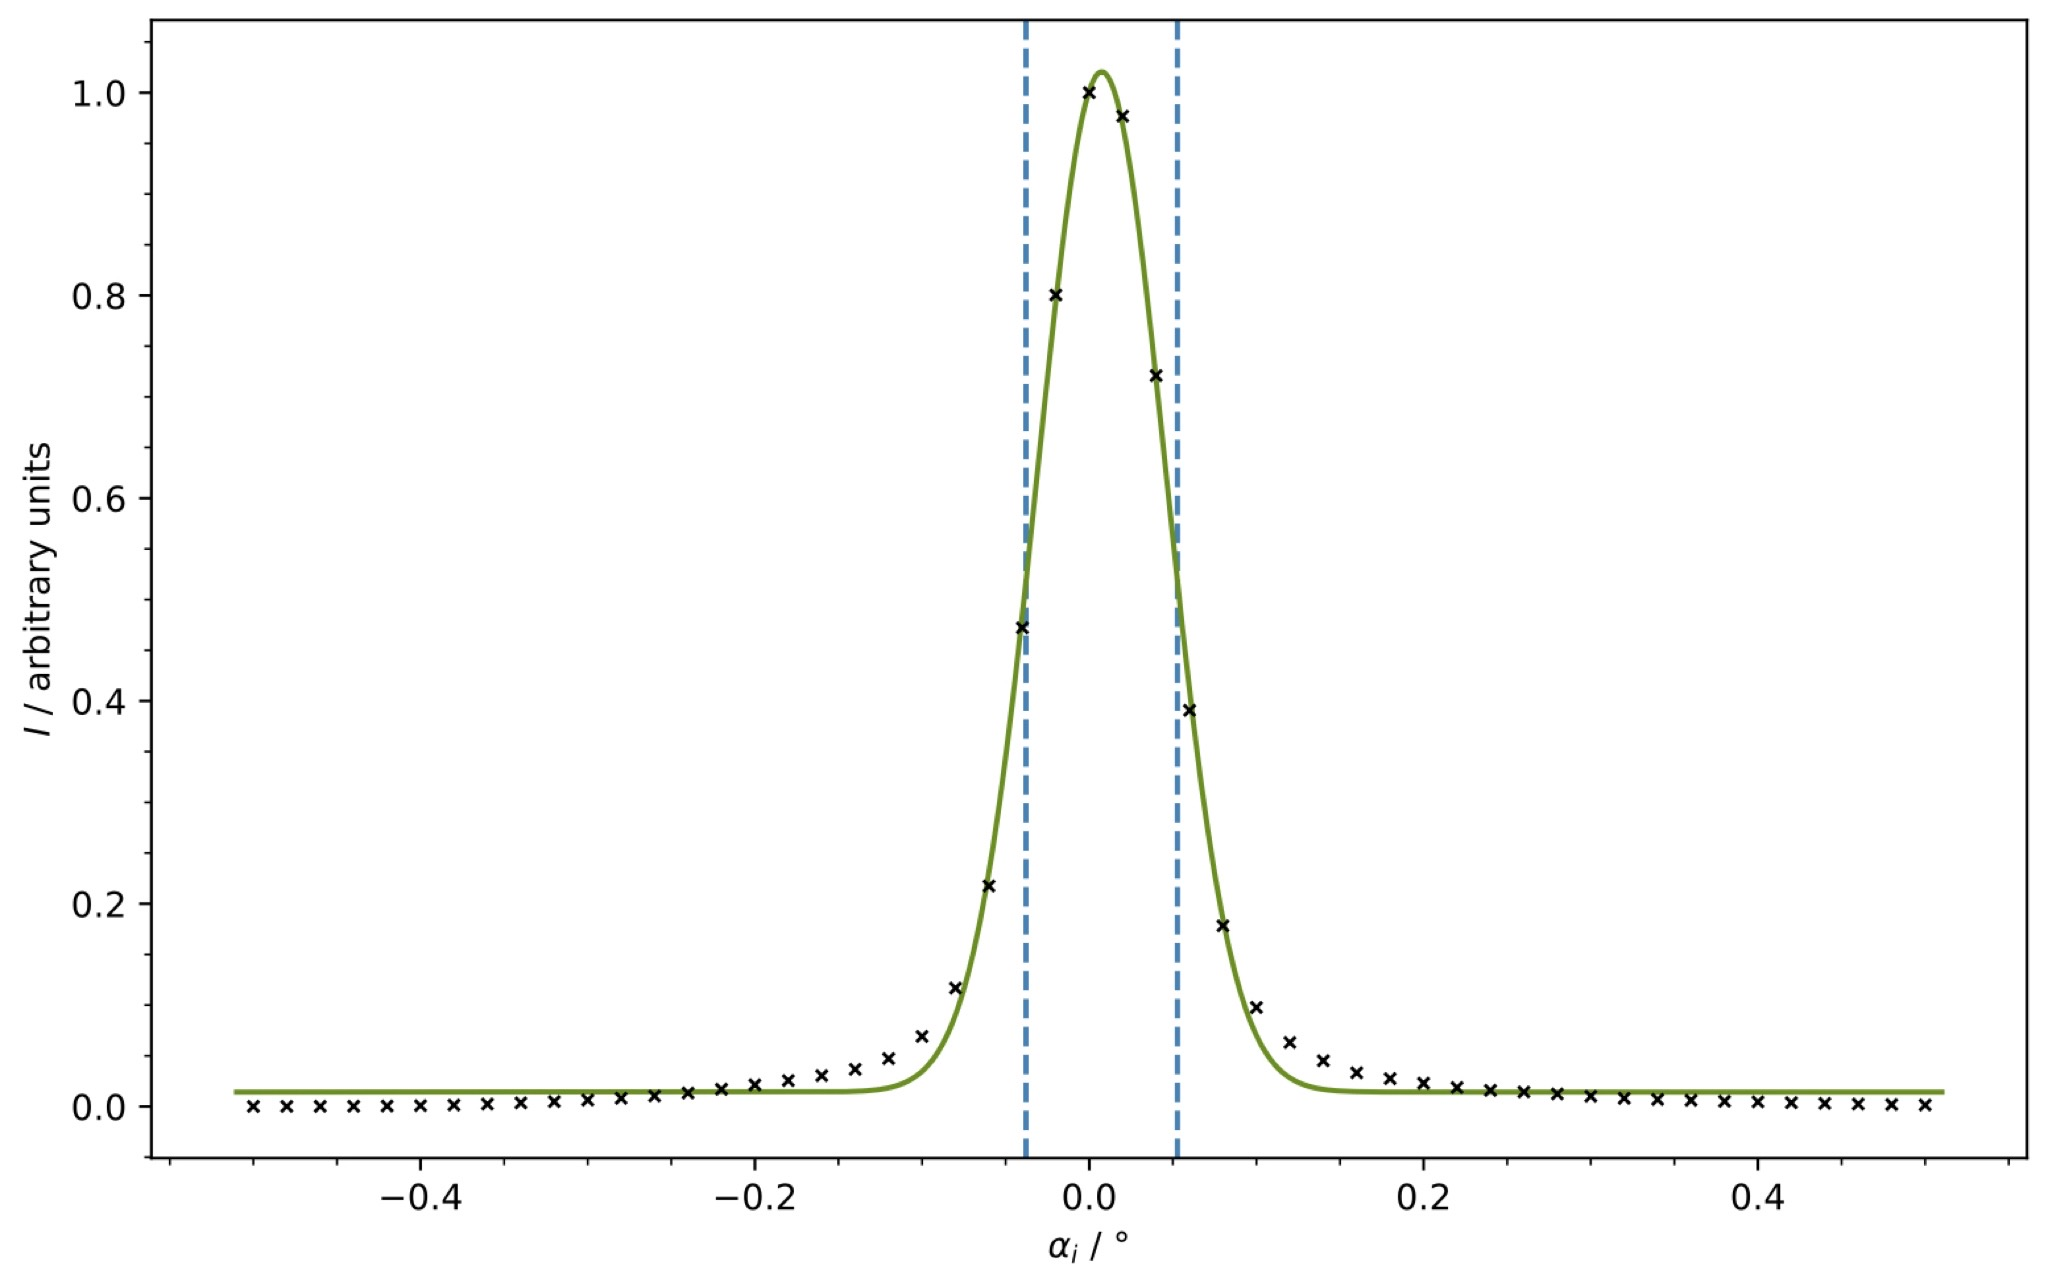
\includegraphics[width=0.88\textwidth]{content/plots/1.jpg}
	\caption{Detector-Scan with fitted Gaussian and marked half maximum positions.}
	\label{fig:detector-scan}
\end{figure}

The curve fit to this function shown in Figure \ref{fig:detector-scan} yields parameters
\begin{align*}
	a &= \num{1.01+-0.01} \: , & b &= \num{0.014+-0.002} \: , \\
	\mu &= \qty{0.0074+-0.0004}{\degree} \: , & \sigma &= \qty{0.0385+-0.0005}{\degree} \: .
\end{align*}
One then finds the maximum at $\alpha_{i, \text{max}} = \mu$ as $G(\alpha_{i, \text{max}}) = \num{1.02+-0.01}$
and full width half maximum at $\alpha_{i, \text{fwhm}}^\pm = \mu \pm \sigma \sqrt{2 \ln 2}$ with
\begin{align*}
	\alpha_{i, \text{fwhm}}^+ = \qty{-0.0528+-0.0007}{\degree} \: , &&
	\alpha_{i, \text{fwhm}}^- = \qty{-0.0379+-0.0007}{\degree} \: .
\end{align*}
Following the detector calibration, the sample position is adjusted. When adjusting the vertical coordinate, one identifies the difference
between maximum to minimum intensity, representing zero to full beam obstruction, with the beam width. As indicated in Figure~\ref{fig:z-scan},
a value
\begin{equation*}
	\tilde{d} = \qty{0.24+-0.06}{\milli\meter}
\end{equation*}
is determined.

\begin{figure}[H]
	\centering
	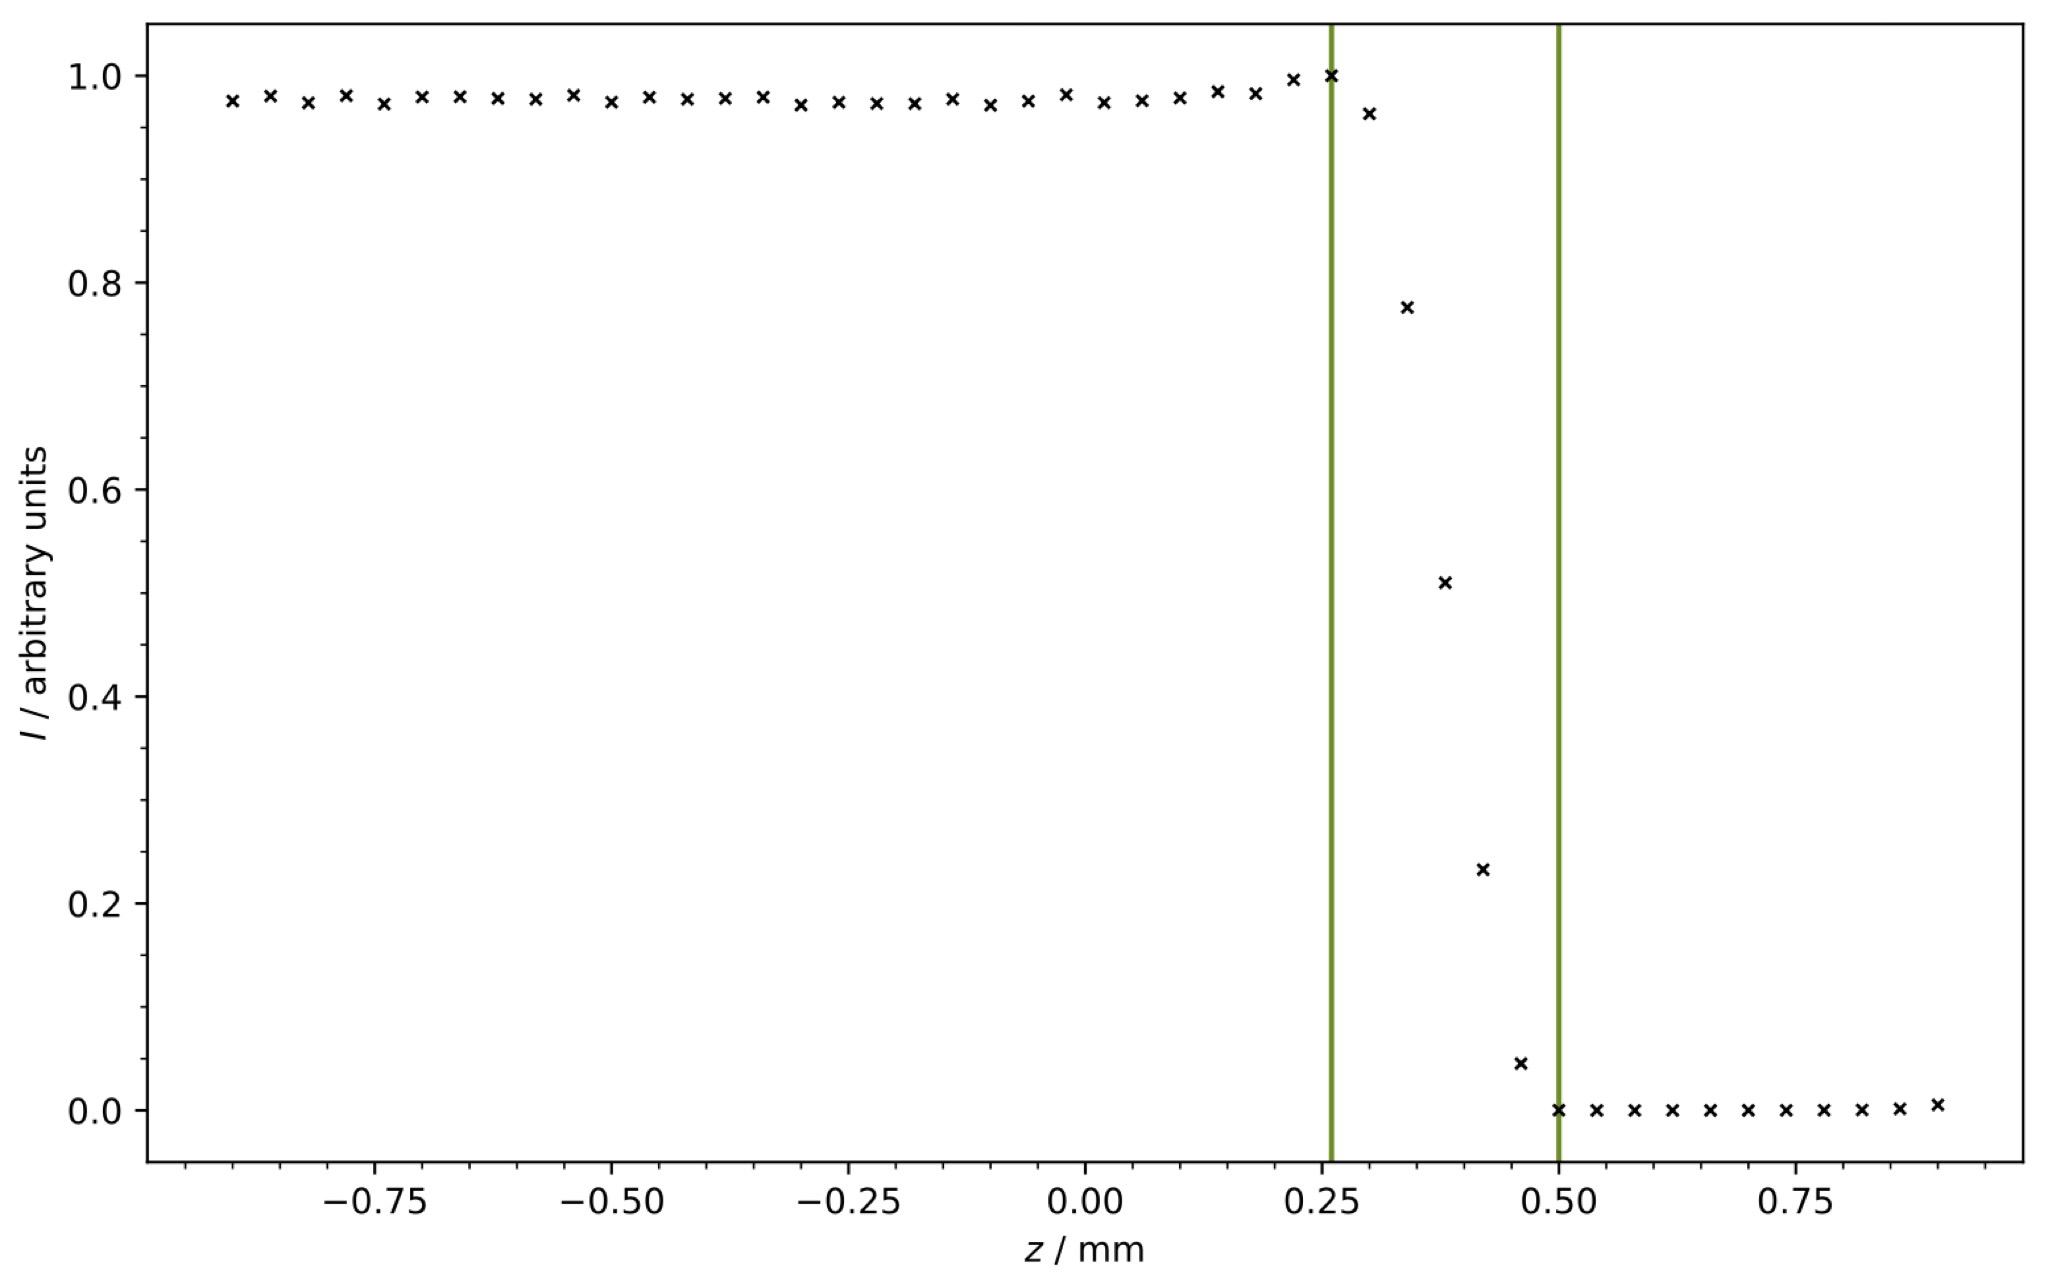
\includegraphics[width=0.88\textwidth]{content/plots/2.jpg}
	\caption{Z-Scan with indicated beam width.}
	\label{fig:z-scan}
\end{figure}

From the intensity valley during horizontal shifting, Figure \ref{fig:x-scan} leads to a sample size
\begin{equation*}
	D = \qty{21+-3}{\milli\meter} \: ,
\end{equation*}
which is in agreement with the literature value $D = \qty{20}{\milli\meter}$ \cite{xray}. From equation \eqref{eqn:geom-angle} follows a
geometry angle
\begin{equation*}
	\alpha_{g, 1} = \qty{0.7+-0.2}{\degree} \: .
\end{equation*}
Reading the geometry angle from Figure \ref{fig:rocking-curve}, a somewhat lower value of
\begin{equation*}
	\alpha_{g, 2} = \qty{0.54+-0.03}{\degree}
\end{equation*}
is obtained, though it still falls inside the uncertainty of the previous result.

\begin{figure}[H]
	\centering
	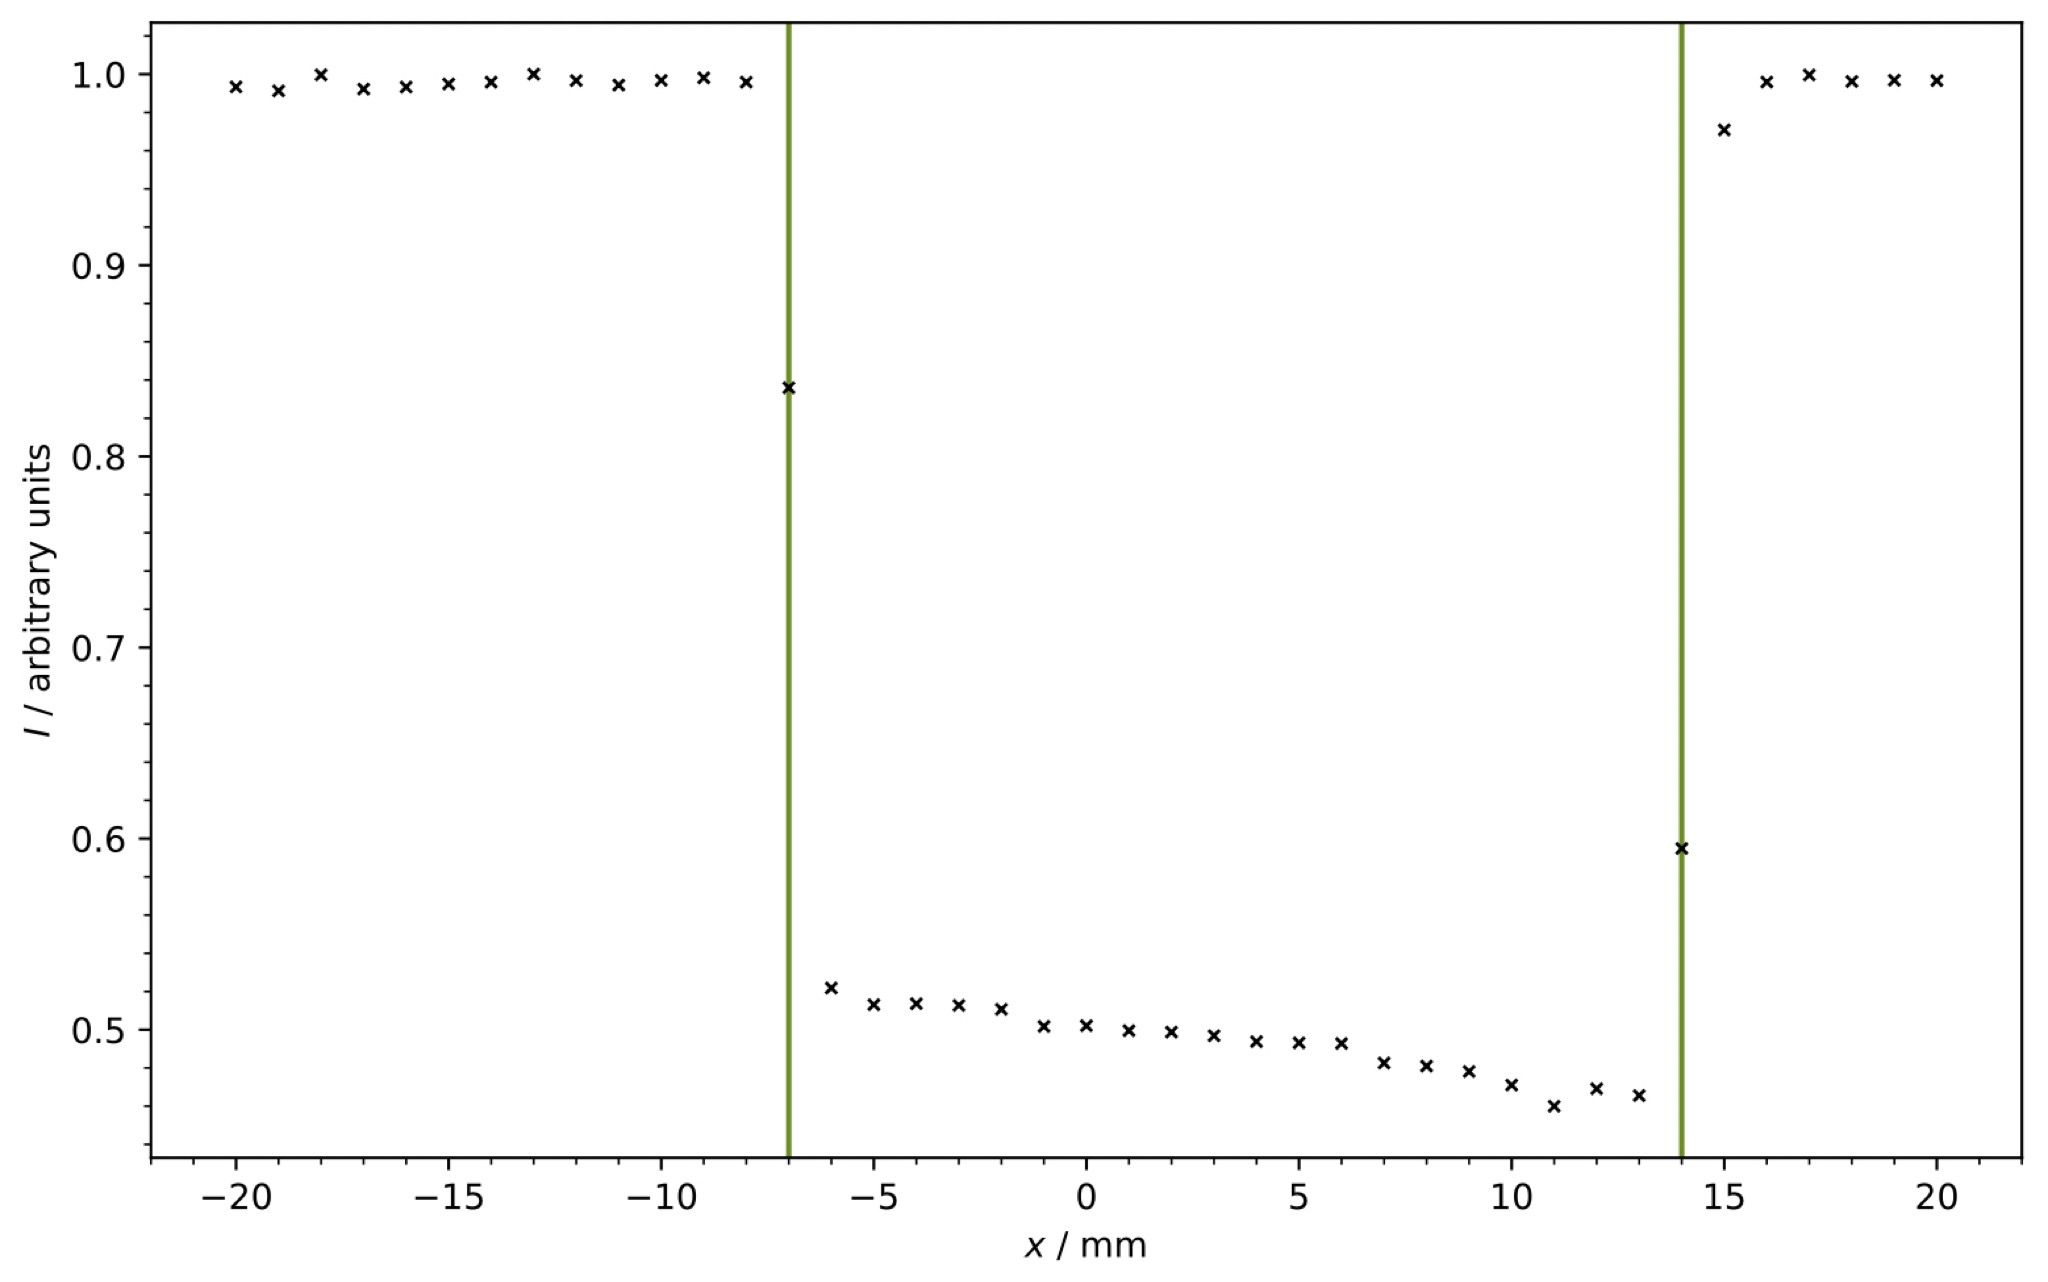
\includegraphics[width=0.88\textwidth]{content/plots/3.jpg}
	\caption{X-Scan with indicated sample size.}
	\label{fig:x-scan}
\end{figure}

\vspace{3em}

\begin{figure}[H]
	\centering
	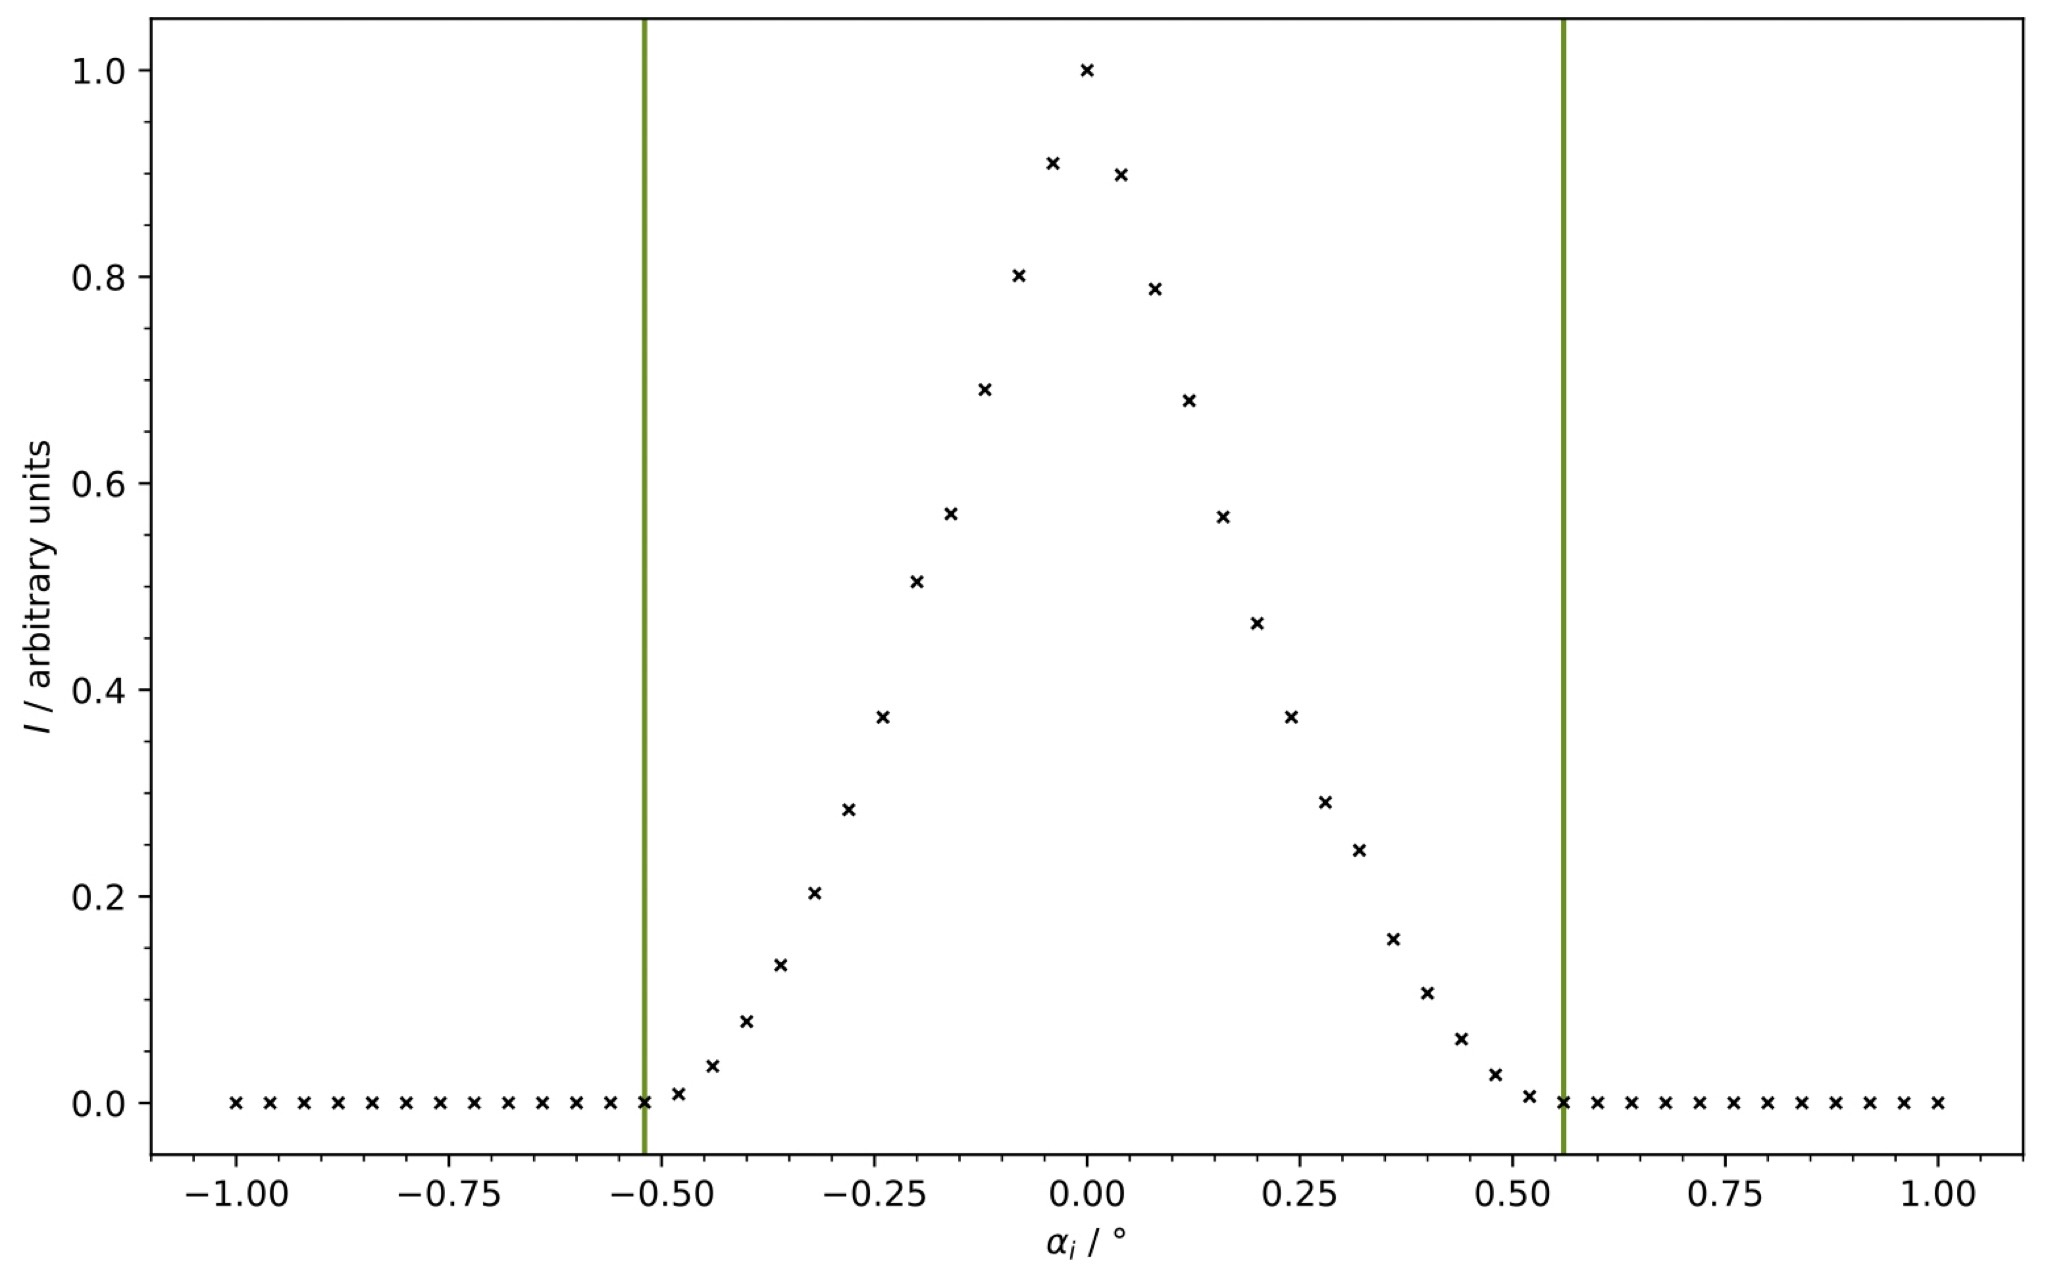
\includegraphics[width=0.88\textwidth]{content/plots/4.jpg}
	\caption{Rocking-Curve with geometry angles.}
	\label{fig:rocking-curve}
\end{figure}



\subsection{Measurement}

Having completed the adjustments, raw data from the diffusive scan is subtracted from the reflectivity scan to correct for scattering
effects which otherwise decrease the signal to noise ratio. This step is depicted in Figure \ref{fig:reflex-diffuse}.

\begin{figure}[H]
	\centering
	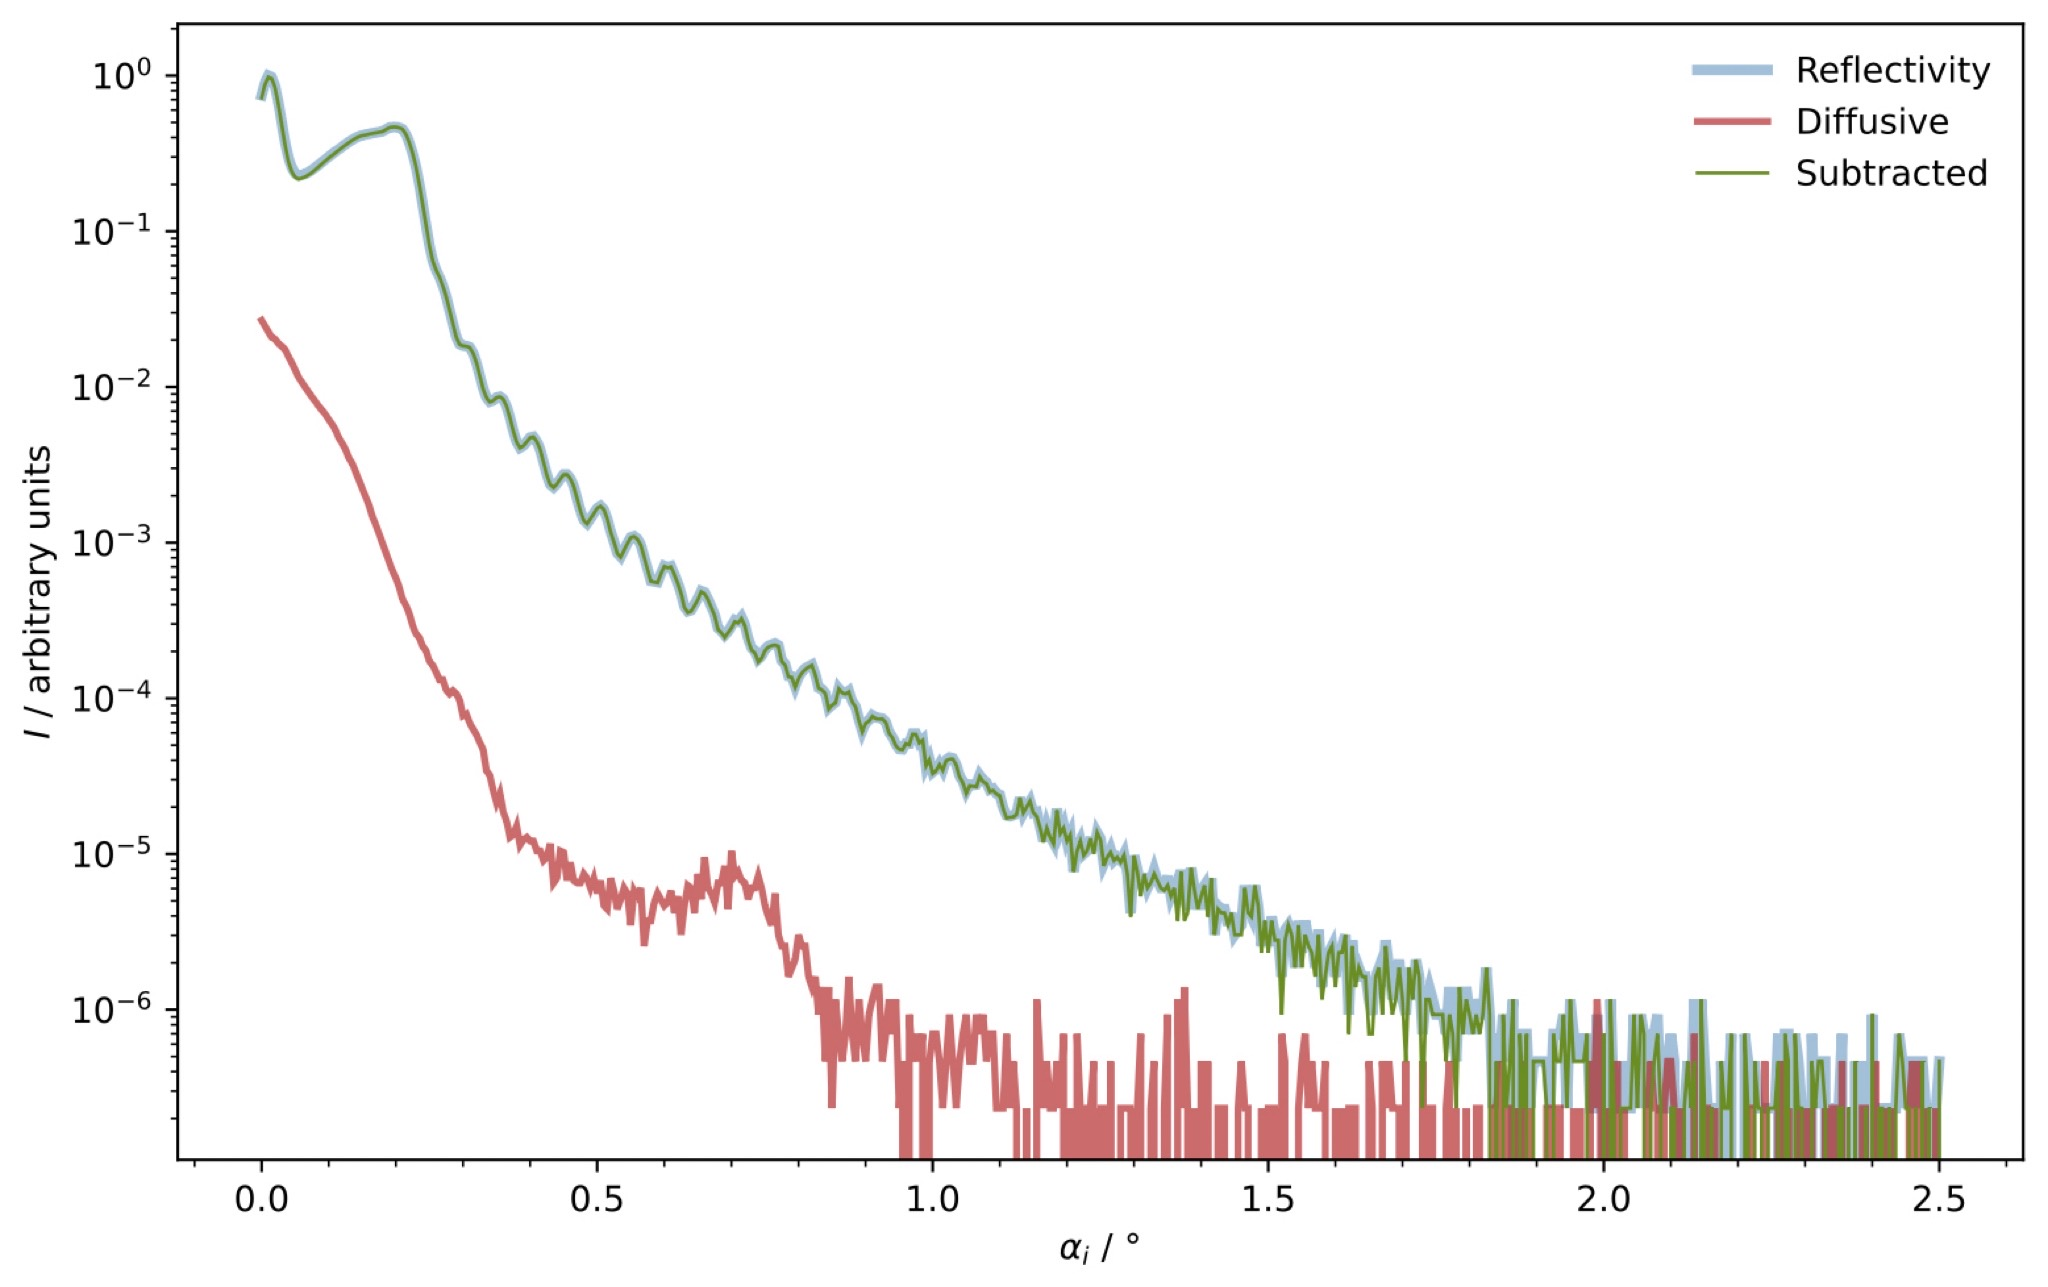
\includegraphics[width=0.88\textwidth]{content/plots/5.jpg}
	\caption{Intensity curves for reflectivity and diffusive background.}
	\label{fig:reflex-diffuse}
\end{figure}

Proceeding from this, the calculated intensity is divided by the geometry factor \eqref{eqn:geom-factor} to correct for less than complete
beam obstruction. The resulting curve is displayed in Figure \ref{fig:geom-corr} and shows a plateau of total reflection below a critical
angle
\begin{equation*}
	\alpha_{c} = \qty{0.21+-0.01}{\degree} \: .
\end{equation*}
The shaded region represents unity reflectivity $R = 1$ and therefore allows one to use the average intensity in this range
$I = \num{1.8+-0.2}$ as a normalization factor. Identifying $\alpha_c \cong \sqrt{2\delta}$, the dispersion
\begin{equation*}
	\delta = \num{6.4+-0.6e-6}
\end{equation*}
can serve as an initial guess for the corresponding parameters in the recursive Parratt formalism. Additionally,
equation \eqref{eqn:dispersion} can be used to estimate the electron density
\begin{equation*}
	\rho_e r_e = \qty{1.7+-0.2e11}{\per\centi\meter\squared} \: .
\end{equation*}
By evaluating the Kiessig peaks in Figure \ref{fig:kiessig-peaks}, one finds the layer thickness via \eqref{eqn:thick}.

\begin{figure}[H]
	\centering
	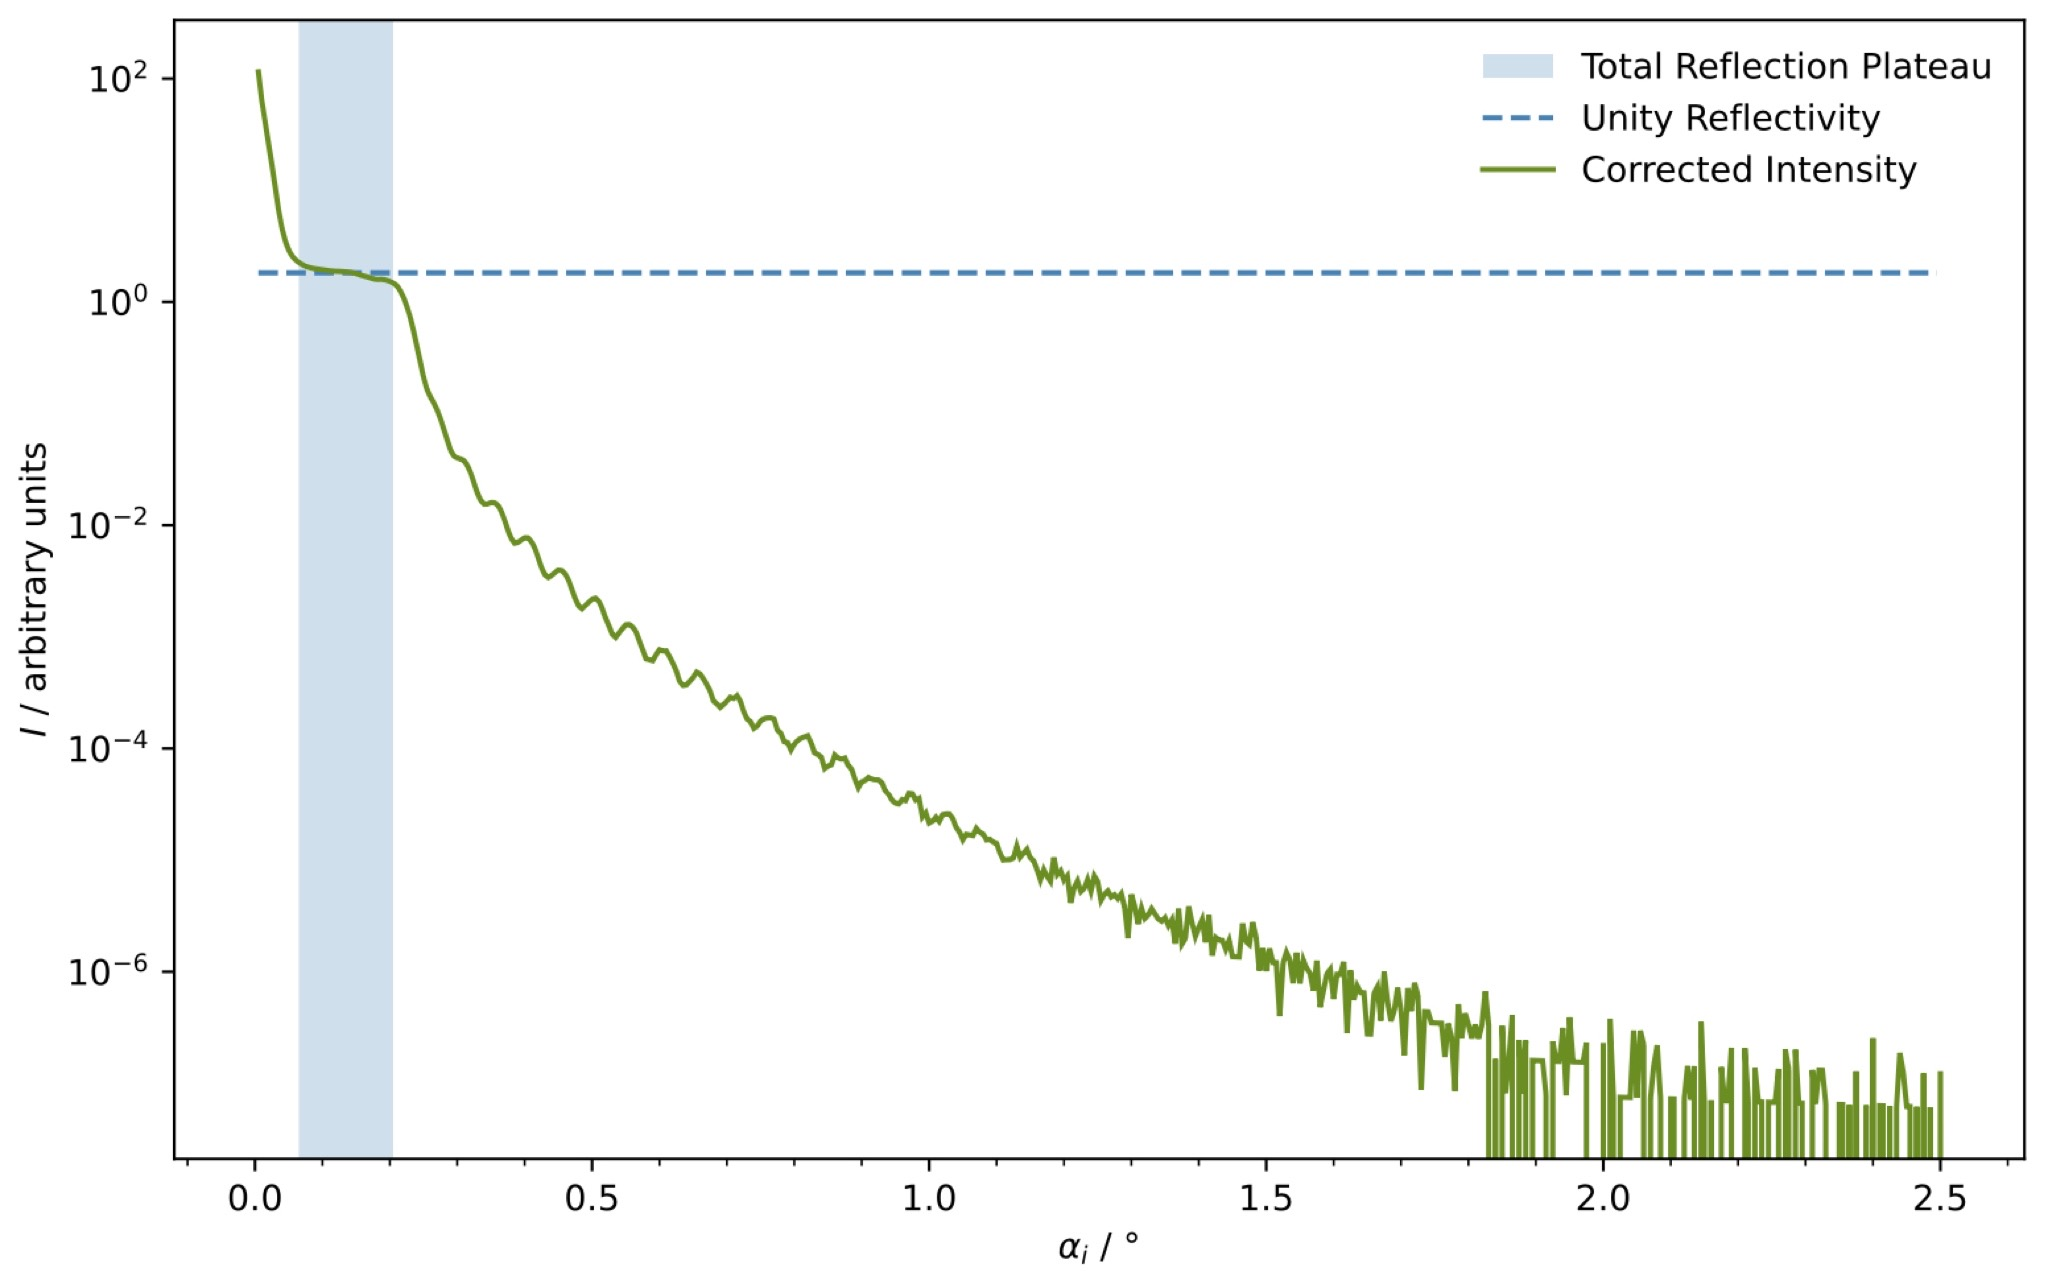
\includegraphics[width=0.88\textwidth]{content/plots/6.jpg}
	\caption{Intensity after geometry factor correction and region of total reflection.}
	\label{fig:geom-corr}
\end{figure}

\vspace{3em}

\begin{figure}[H]
	\centering
	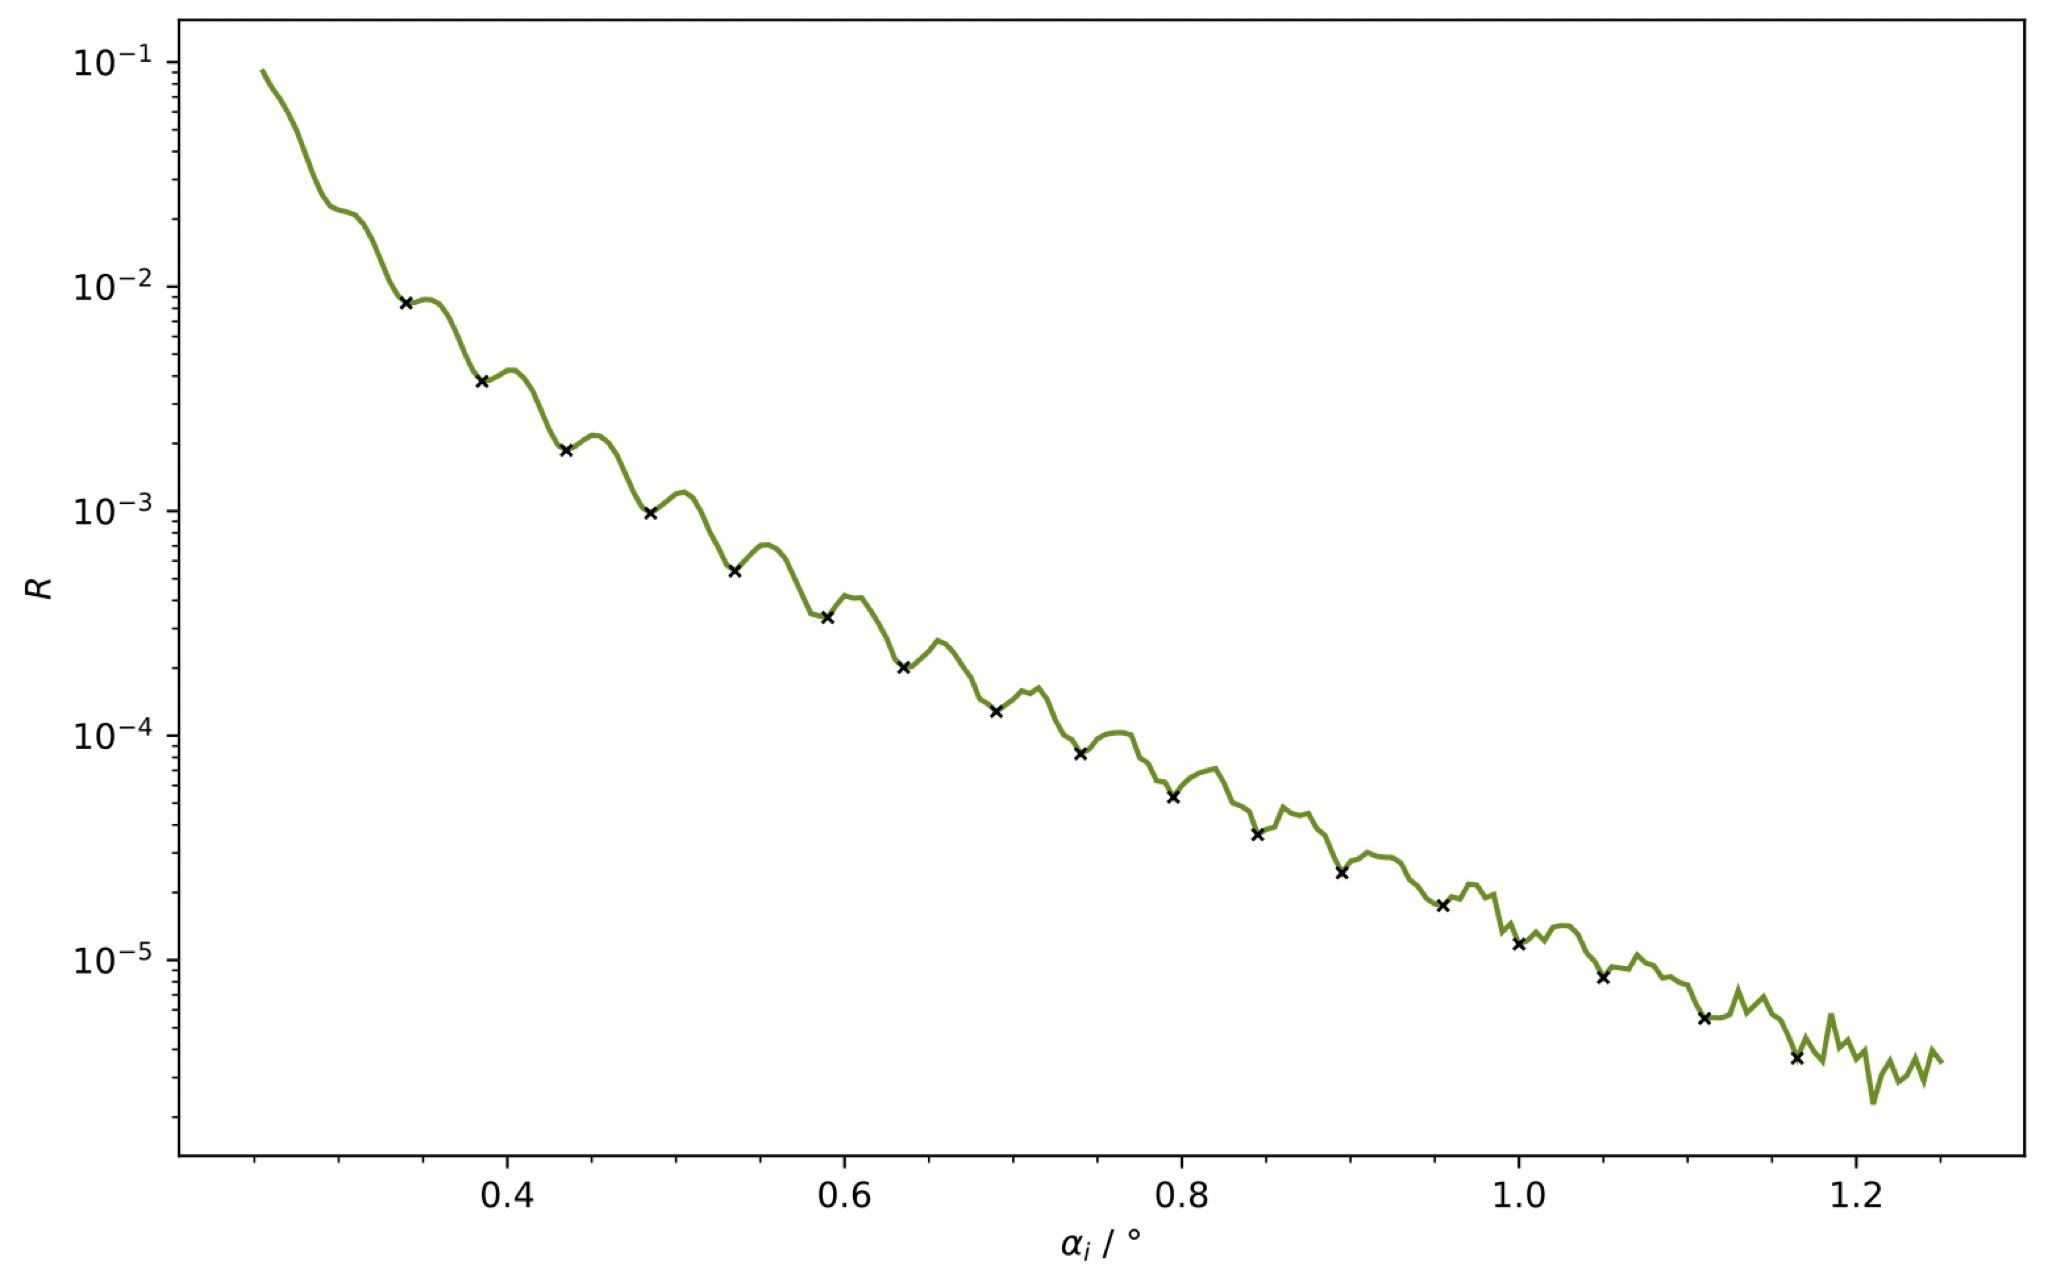
\includegraphics[width=0.88\textwidth]{content/plots/7.jpg}
	\caption{Detailed reflectivity curve with Kiessig oscillation minima.}
	\label{fig:kiessig-peaks}
\end{figure}

\newpage

To this end, the average angular distance $\Delta \alpha_i = \qty{0.052+-0.005}{\degree}$ between adjacent minima with wavelength
$\lambda = \qty{1.5406e-10}{\meter}$ for the $\text{Cu } K_\alpha$ emission line yields
\begin{equation*}
	d = \qty{8.6+-0.8e-8}{\meter} \: .
\end{equation*}
Finally, Figure \ref{fig:parratt-fresnel} includes two fits to the observed reflectivity. First, a Fresnel curve for an ideally smooth
$\text{Si}$ surface is plotted according to \eqref{eqn:fresnel} with parameters
\begin{align*}
	\delta = \num{7.6+-2.3e-6} \: , && \beta = \num{0.0+-0.4e-6} \: .
\end{align*}
Furthermore, a manual optimization of the Parratt algorithm is performed based on the previously obtained input quantities, arriving at
\begin{align*}
	\delta_1 &= \num{7.3e-7} \: , & \delta_2 &= \num{6.6e-6} \: , \\
	\beta_1 &= \num{4.1e-9} \: , & \beta_2 &= \num{1.6e-7} \: , \\
	\sigma_{01} &= \qty{8.3e-10}{\meter} \: , & \sigma_{12} &= \qty{8.1e-10}{\meter} \: , \\
	d_1 &= \qty{8.6e-8}{\meter} \: .
\end{align*}
From these, one finds
\begin{align*}
	\alpha_{c, 1} &= \qty{0.069}{\degree} \: , & \alpha_{c, 2} &= \qty{0.208}{\degree} \: ,\\
	\rho_{e, 1} r_e &= \qty{1.93e10}{\per\centi\meter\squared} \: , &
	\rho_{e, 2} r_e &= \qty{1.75e11}{\per\centi\meter\squared} \: .
\end{align*}

\begin{figure}[H]
	\centering
	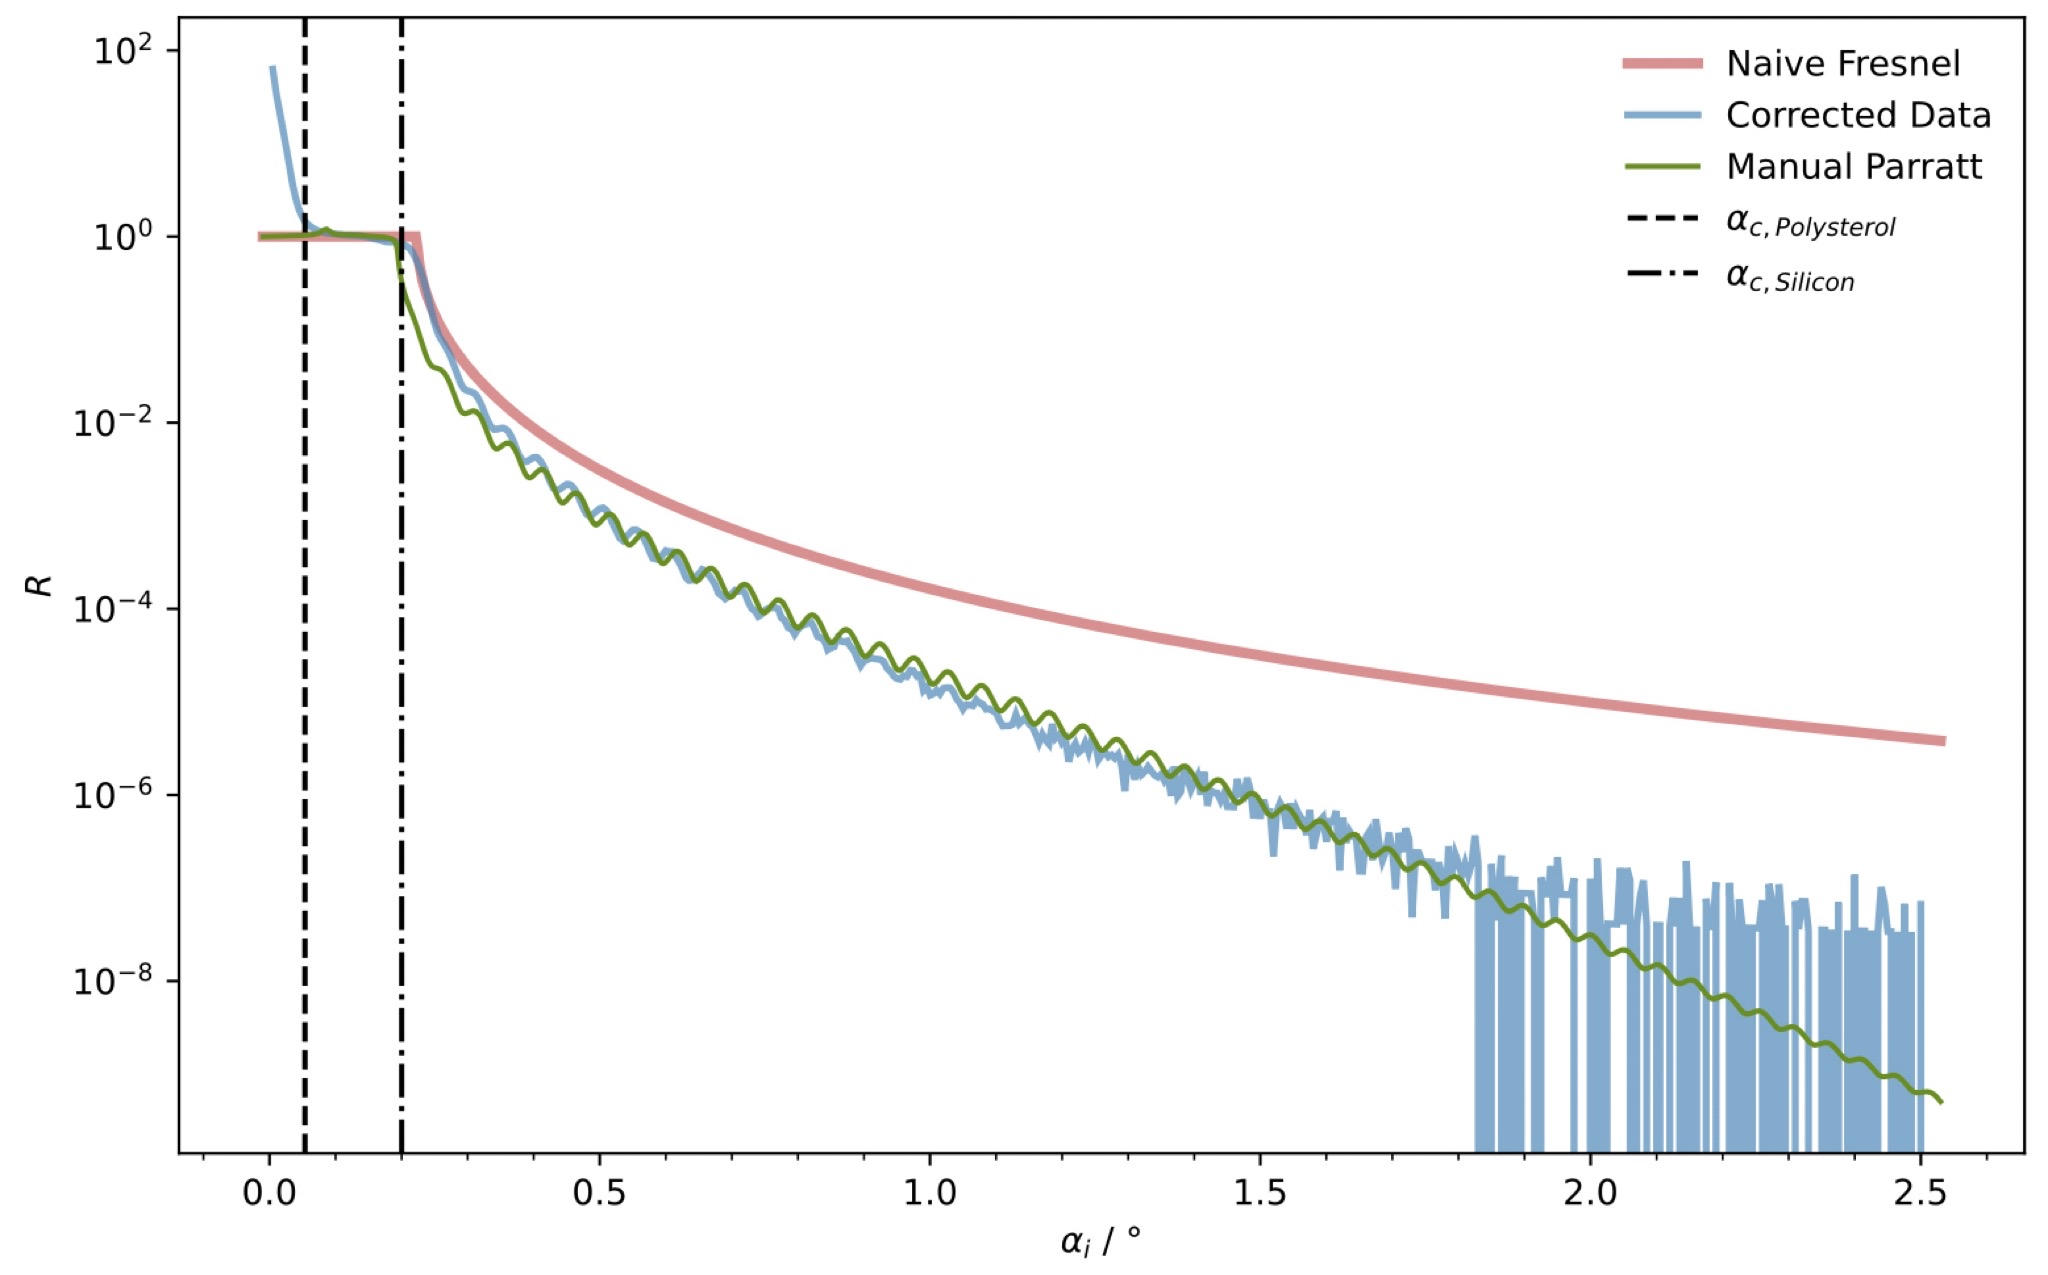
\includegraphics[width=0.88\textwidth]{content/plots/8.jpg}
	\caption{Full reflectivity curve with Parratt and Fresnel fits.}
	\label{fig:parratt-fresnel}
\end{figure}
